%%%%%%%%%%%%%%%%%%%%%%%%%%%%%%%%%%%%%%%%%%%%%%%%%%%%%%%%%
\chapter[Présentation d’eLua]{Présentation d’eLua}
\label{chap:chap3}

\section{À propos de Lua}

Lua est un langage de script libre, réflexif et impératif. Il a été conçu afin de pouvoir être embarqué au sein d'autres applications et les étendre.
Lua (qui signifie lune en portugais) a été développé par des membres du groupe de recherche TeCGraf, de l'université de Rio de Janeiro au Brésil.
Il est écrit en langage C ANSI strict, et de fait, il est compilable sur une grande variété de systèmes; et le plus souvent utilisé dans des systèmes
embarqués, car sa compacité est très appréciée. De plus, il possède une compatibilité avec le langage C, c'est-à-dire qu'il est facile d'écrire du code
C et de l'exécuter dans des scripts Lua). Lua a déjà été utilisé pour le développement de jeux vidéo (beaucoup de jeux 2D de développeurs indépendants)
ou encore comme langage de configuration du jeu World of Warcraft de Blizzard Entertainment.

\begin{figure}[h]
\begin{center}

\includegraphics[scale=1]{../images/eLua/Lua.JPG}
\caption{Logo Lua}
\end{center}
\end{figure}


\section{Qu'est-ce qu'eLua?}

  eLua adopte le langage de programmation Lua et propose une implémentation complète de celui-ci pour les systèmes embarqués. Il ajoute au langage de base,
une API spécifique à ces systèmes pour rendre le développement de logiciels embarqués plus simple.

\subsection{Architecture de eLua}

\begin{figure}[h]
\begin{center}
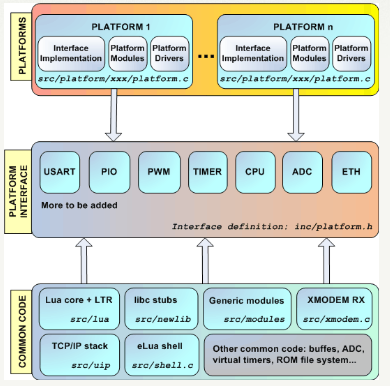
\includegraphics[scale=0.6]{../images/eLua/schema.png}
\caption{Structure logique de eLua}
\label{elua}
\end{center}
\end{figure}

  Dans la documentation d'eLua on utilise la notion de ``plateforme'' pour désigner un groupe de CPU qui partagent la même structure du noyau; pourtant
ils peuvent différer dans le nombre de péripheriques integrés, la mémoire interne, et tout autre attribut. Un port eLua implémente un ou plusieurs
CPU d'une même plateforme.
Dans la figure~\ref{elua}, on observe que eLua essaie d'être aussi portable que possible dans différentes plateformes, pour cela plusieurs règles ont été mises en
place, entre autres :

\begin{itemize}
 \item Le code qui est indépendant du type de plateforme doit être écrit en ANSI C dans toutes les parties où cela est possible, afin qu'il soit
portable parmi plusieurs architectures et compilateurs, comme Lua.

 \item Le code qui ne peut pas être générique (par exemple le péripherique et le code spécifique au CPU) doit être aussi portable que possible en
utilisant une interface en commun qui doit être implementée par toutes les plateformes dans lesquelles eLua peut être executé.

 \item Toutes les plateformes et leur péripheriques ne sont pas créés de la même façon et possèdent donc des fonctionnalités très variées. Pour accéder
à une fonctionnalité spécifique à une plateforme on peut utiliser un module. Ces modules ont été créés afin de compléter l'écart entre l'interface de
la plateforme et toutes les caractéristiques proposées par la plateforme.

\end{itemize}

\subsection{Code en commun}

La liste suivante montre quelques éléments qui sont classifiés comme du code en commun :

\begin{itemize}
 \item Le code Lua
 \item Tous les composants eLua (par exemple le ROM file system, le shell eLua, et autres)
 \item Tous les modules génériques, qui sont des modules exportés de Lua
 \item Le code générique des périphériques
\end{itemize}

C'est important de remarquer que les parties génériques doivent être la grande partie du code. Par exemple, lorsqu'on veut ajouter un nouveau fichier au système
celui-ci doit être un code générique, sinon le code aura des dépendances par rapport à l'emplacement où il réside. On peut corriger cela en utilisant des fonctions
définies dans l'interface de la plateforme, mais si cela n'est pas possible il faudra séparer les fonctions spécifiques dans une interface séparée qui va
devoir être implémentée par toutes les plateformes qui veulent utiliser ce nouveau fichier. Ceci donne un maximum de portabilité au code.

L'utilisateur ne doit jamais oublier le but principal de eLua : la flexibilité. Il doit donc être dans la capacité de savoir quels composants font partie
de son binaire eLua.

\section{Avantages de eLua}

\begin{description}

 \item[Contrôle total de la plateforme:] il n'existe pas un systèmee d'exploitation entre les programmes et le microcontrôleur.

 \item[Portabilité du code:] Comme Lua, le programme peut être exécuté dans un grand nombre de plateformes et d'architectures.

 \item[Facilité de transformation:] Le code et la conception des applications pour eLua peuvent être indépendants du matériel.

 \item[Développement autonome:] Lua est complètement fonctionnel avec la possibilité d'avoir un shell dans le microcontrôleur, il n'y a besoin
de rien installer côté ordinateur à part la connexion du port. Les programmes sont utilisables directement sur la carte microcontrôleur.

 \item[Flexibilité:] L'utilisation de ce Lua comme langage de script de haut niveau dans un projet rend celui-ci très adaptable, facilement
reprogrammable et reconfigurable. Les systèmes sont très efficients pour une future évolution.

 \item[Apprendre l'embarqué: ] L'expérimentation est très simple et interactive.

 \item[Open Source:] elua est libre, gratuit, et open source, comme Lua, il possède une licence MIT.
\end{description}




